%----------------------------------------------------------------------------
%\chapter{\Kubernetes}
%\label{sec:Kubernetes}
%----------------------------------------------------------------------------
\chapter{Kubernetes}
\label{sec:Kubernetes}
A diplomamunka keretén belül végzett feladataim jelentős részben támaszkodnak a Kubernetes (\textit{K8s}) rendszerre, így annak alapvető ismertetése szükségszerű a dolgozat további megértéséhez.
Egy rendkívül széleskörű platformról van szó, szerteágazó felhasználási területekkel, emiatt a rendszer teljes és mély ismertetésére helyett próbáltam a dolgozat szemszögéből ténylegesen szükséges információk körére szorítkozni.

%----------------------------------------------------------------------------
\section{Kubernetes motivációja és rövid története}
%----------------------------------------------------------------------------
Ahogy egyre többen kezdték megismerni és alkalmazni a konténerizációs technológiákat, úgy vált egyre hangsúlyosabbá az üzemeltetési oldalon is.
A korábbi kihívások átalakultak a technológia változásával együtt. 
Ezek után már nem az egyes szerverek vagy virtuális gépek (\textit{VM}) adminisztrációs terhe jelentette a kihívást, hanem annak a számos mozgó alkatrésznek a kezelése, amelyből egy modern alkalmazás felépült.
Ugyanis a részegységekre bontásnak a következményeként sok kis konténert kell egyszerre felügyelni, ami jelentősen több feladattal jár, mint a korábbi VM alapú, monolitikus rendszerek kezelése esetén.
%Az új igények szerint az alkalmazás egyes részei egymástól függetlenül, külön konténerekben futnak.
%Ezáltal sokkal több kisebb részegység felügyelete vált szükségessé, ami jelentősen több feladattal jár, mint a korábbi fizikai vagy virtuális gépek adminisztrációs terhei. 

Ez a probléma motiválta a Google szakembereit is, hogy egy olyan új platformot fejlesszenek, ami képes a fenti kihívások megoldására.
Eleinte a projekt a \textit{Borg}\citep{Borg} nevet viselte, amit aztán 2014-ben a Google nyílt forráskódúvá tett Kubernetes néven.
A projektet a \textit{Cloud Native Computing Foundation (\textit{CNCF})}\citep{cncf} vette gondozásába.
Innentől kezdve bárki szabadon elérheti és fejleszthet is bele.
Az elmúlt 6 év alatt hatalmas fejlődésen ment keresztül és már a $22$.-ik kiadásánál tart.

Egészen fiatal rendszerről van tehát szó, azonban a VMware kutatásából\citep{VMwareSurvey} is sok érdekes dolog derül ki.
Egyre többen térnek át a Kubrenetesre és futtatják benne a konténerizált alkalmazásaikat. 
Látható, hogy nem egy rövidtávon elmúló trendről van szó és még mindig felívelő ágban van, a korábbi alternatívák fokozott kiszorításával.
A kutatásban résztvevők jelentős része számolt be hatékonyság növekedésről, főként az erőforrás gazdálkodásban és a fejlesztési ciklusok rövidítésének tekintetében.

Ma már gyakorlatilag a Kubernetes a konténer orkesztráció szinonimája és egyeduralkodó a területén, azonban ez nem mindig volt így.
Az alapvető problémát, hogy meg kell könnyíteni a konténerek kezelését sokan felismerték és több megoldás is született rá. 
A különböző eszközök és fejlesztések közötti versenyt konténer orkesztrációs háborúnak is nevezik\citep{containerOrchestrationWar}, melynek egyedüli győzteseként a Kubernetes került ki.

%----------------------------------------------------------------------------
\section{Felépítése}
%----------------------------------------------------------------------------

\subsection{Architektúra}
%----------------------------------------------------------------------------
Kubernetes alatt általában egy teljes klasztert szoktak érteni, ami sokrétű problémára jelent megoldást.
Feladatai közé tartozik a konténerek elindítása, azok felügyelete, kezelése. 
Ezenfelül kezeli a konténerek közti hálózatot, irányítja a forgalmat.
A feladatok ellátásában több különböző egység vesz részt, saját hatáskörökkel. 
Az alábbi fejezetben szeretném ezeket az egységeket bemutatni és átfogó képet adni a Kubernetes működéséről.  

\subsubsection{Csomópontok}
A legtöbb klaszter több csomópontból (\textit{node}) épül fel, mely egy teljes fizikai szervert vagy egy virtuális gépet jelent a gyakorlatban.
Itt fognak futni a később részletesen tárgyalt kapszulák (\textit{pod}\footnote{A diplomamunka során felváltva használom az angol és magyar nyelvű kifejezéseket, hogy kevésbé legyen szóismétlő; illetve az angol megfelelő a beszélt közegben gyakoribb, viszont írásban a ragozása nehéz feladat.}), mely a Kubernetes legkisebb egységei és egy vagy több konténert tartalmazhatnak.
Ezért itt szükség van azoknak a szolgáltatásoknak, amik ezt lehetővé fogják tenni.
A csomópontok konfigurációját a vezérlő sík (\textit{control plane}) végzi, melyről szintén részletesen lesz szó \aref{subsec:controlplane} alfejezetben.
A \ref{k8s_nodes} sorszámmal ellátott kódrészleten láthatjuk, hogy az általunk későbbiekben használt klaszter esetében milyen csomópontok vannak.
Fontos, hogy az egyes node nevek  különbözőek legyenek. 

Feladatkörét tekintve két különböző típusú node lehet.
Egyik, ami a vezérlő síkot biztosítja, az úgynevezett \textit{master} illetve a másik, ahol csak kapszulák futhatnak, ezek a \textit{worker} típusú csomópontok.
Látható, hogy a példaként hozott kódrészletben a \verb+dipterv1+ névvel ellátott node van mester szerepben.
Az utóbbi időben egyre jobban elmosódott a határvonal a két típus között.
Ajánlottan a master komponensek külön, dedikált csomópontokon futnak, de szabadon konfigurálható és akár futtathatunk alkalmazás specifikus kapszulákat is rajtuk.\\
% és több csomóponton van megvalósítva a vezérlő sík, illetve ezeken is lehet kapszulákat futtatni.

\lstset{caption=Később használt klaszter csomópontjai, label=k8s_nodes}
\lstinputlisting{figures/kubectl_get_nodes.sh}

A kapszulák futtatásához a Kubernetesnek lehetővé kell tenni a podok indítását az egyes csomópontokon és a közöttük lévő kommunikációt. 
Ezért minden egyes node rendelkezik az alábbi komponensekkel:

\paragraph{Kubelet} Minden node rendelkezik egy \textit{kublet} nevű ügynökkel (\textit{agent}), mely feladata az adott csomópontra ütemezett konténerek rend szerinti futtatása. 
A futtatandó parancs a vezérlő sík felől érkezhet (a Kubernetes API szerverén keresztül), egy úgynevezett pod leíró kíséretében, amelyben lévő definíció alapján kezeli a \textit{kubelet} a kapszulákat. Ez az alsóbb szinteken azt jelenti, hogy elindítja a szükséges konténereket a csomóponton.
Ezen felül feladata, hogy az általa összegyűjtött információkat jelentse a vezérlő sík felé, ezzel lehetővé téve az új konténerek ütemezési döntését a csomópontokra. 

\paragraph{Kube-proxy} A \textit{kube-proxy} szintén része minden csomópontnak, ahogy az a \ref{fig:k8s_components} ábrán is látszik. 
Ezen komponens feladata az adott node hálózatát karbantartani.
Ezt úgy tudja megtenni, hogy operációs rendszer szinten hoz létre és kezeli a hálózati csomagokra vonatkozó szabályokat.

\paragraph{Konténert futtató környezet} Mivel az egyes kapszulák konténereket tartalmaznak ezért szükség van egy olyan környezetre, ami képes futtatni ezeket a konténereket.
Mai napig a legelterjedtebb a Docker, de a Kubernetes ezen kívül még több másikat is támogat. 

% Kubernetes cluster components ---------------------------------------------
\begin{figure}[!ht]
\centering
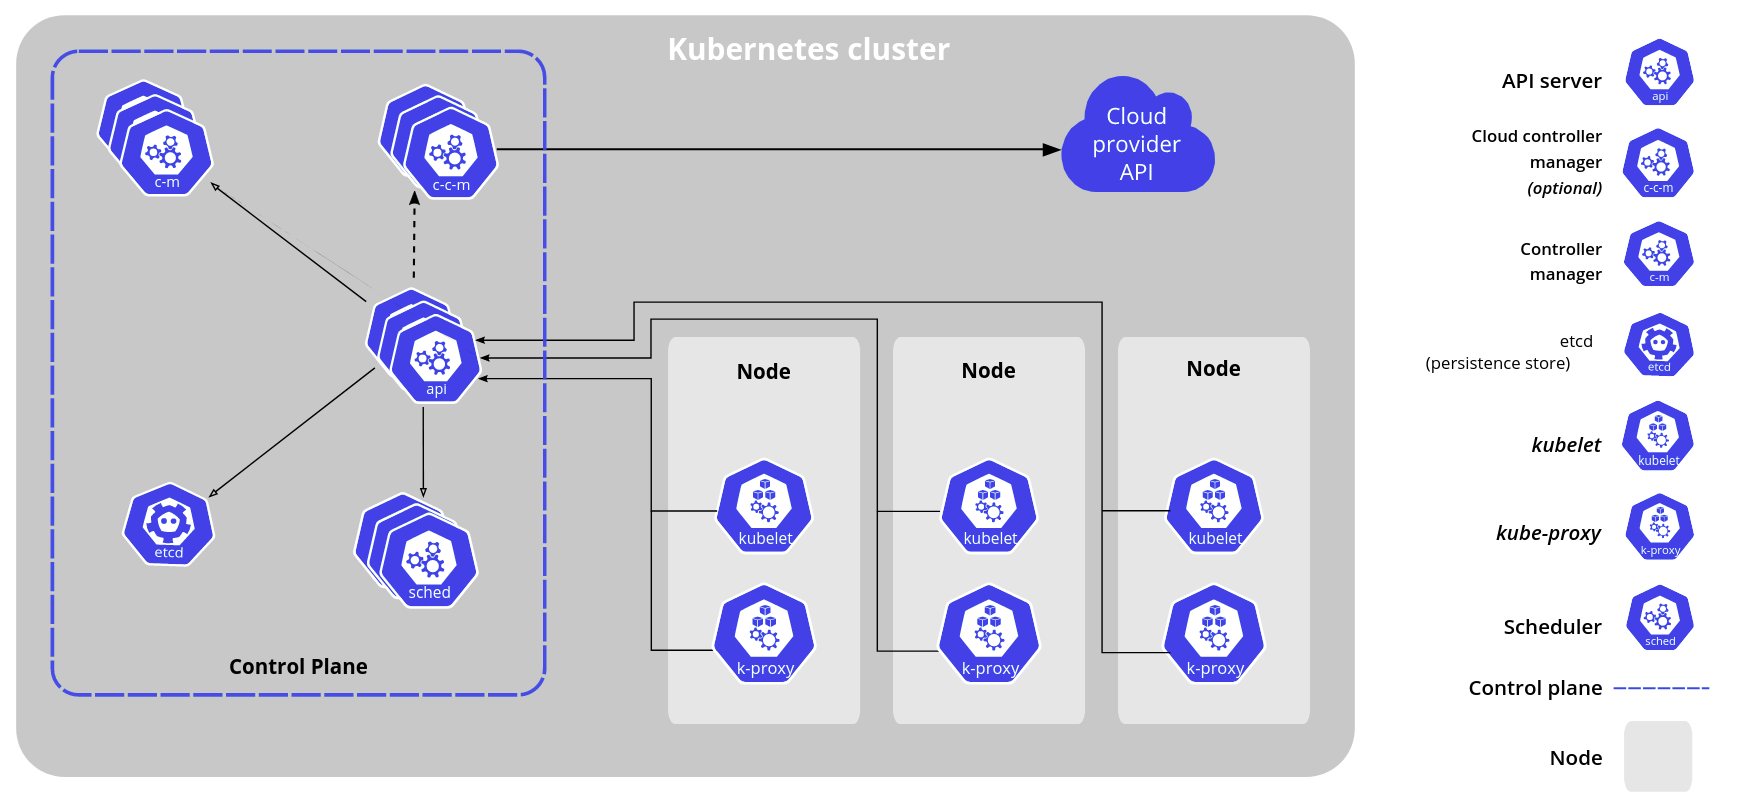
\includegraphics[width=150mm, keepaspectratio]{figures/kubernetes_components.png}
\caption{Kubernetes klaszter elemei\citep{KubernetesComponents}}
\label{fig:k8s_components}
\end{figure}

\subsubsection{Vezérlő sík}
\label{subsec:controlplane}
A Kubernetesen belül a vezérlő sík felelős a klaszteren belüli döntésekért. 
Feladata például meghatározni, hogy az újonnan létrehozandó kapszulák melyik csomóponton induljanak el.
A \ref{fig:k8s_components} ábrán is láthatjuk a vezérlő síkot kék szaggatott vonallal keretezve.

\paragraph{API szerver} A klaszter központi egysége. 
Minden művelet rajta keresztül történik. Felelőssége a beérkező kérések hitelesítése és továbbítása a megfelelő rendszerelemek felé. 
Például a klaszter adminisztrációra használható \verb+kubectl+ parancs használatakor is a parancssori kliens összeállít és elküld egy üzenetet az API szerver felé, ami fogadja és válaszol rá.

\paragraph{Etcd} Az \textit{etcd} komponens is része a vezérlő síknak, ami egy elosztott módon működő\citep{raft} kulcs-érték párokat tartalmazó adatbázist valósít meg.
Itt tárolja a klaszter összes saját tulajdonságát, például az egyes objektumok állapotait is.
Ezáltal a korábbi példaként említett \verb+kubectl+ lekérdezés is ebből az adatbázisból kiolvasott értékeket fogja válaszul megkapni.

\paragraph{Ütemező} Az ütemező (\textit{kube-scheduler}) feladata, meghozni a döntést, hogy egy új pod melyik csomóponton kerüljön létrehozásra.
Ez egy igazán izgalmas feladat, hiszen figyelembe kell vennie a rendszer jelenlegi foglaltságát, illetve a kapszula létrehozásakor külön meg lehet adni megkötéseket a node felé. 
Ilyen megkötés vonatkozhat a csomópont szoftverére vagy hardverére is.  

\subsection{Objektumok}
%----------------------------------------------------------------------------
A Kubernetes egyik erőssége, hogy az átlagos felhasználás esetében nem kell törődni a rendszer felépítésével, hiszen elég deklaratív módon létrehozni az erőforrásokat, objektumokat.
Minden egyéb feladatot a Kubernetes a felhasználók elől elrejtve hajt végre.

\paragraph{Pod (kapszula)}
%\label{par:pod}
A Kubernetesben megjelenő legkisebb logikai egység.
Általában egy konténert tartalmaz, de lehetőségünk van több konténer részletes specifikálására is.
Általánosságban elmondható, hogy rendszeresen létrejönnek és rendszeresen törölve is lesznek ezek az objektumok, tehát nem tartós életűek.
Ezen tulajdonság miatt a rendszer egészére is célszerű egy dinamikusan változó környezetként tekinteni.
Az egyszerű pod kezelése nehéz, mert az állandó változása miatt nincs statikus elérése, nem képes magát skálázni vagy érzékelni az esetleges hibákat. 
Ezen problémákra később látjuk a Kubernetes által nyújtott megoldásokat.

\paragraph{ReplicaSet} 
\textit{ReplicaSet} felelős az általa kezelt kapszulák számának monitorozásáért.
Ennek értelmében, ha az egyik pod meghibásodik és megáll, akkor helyette egy újat fog létrehozni.
Ezáltal biztosított, hogy mindig a megfelelő számú egység fogja fogadni a beérkező kéréseket és nem kell manuálisan monitorozni a státuszukat.
A \textit{ReplicaSet} megoldást nyújt a podok öngyógyulására azáltal, hogy újraindítja a kapszulákat egy esetleges hiba esetén, illetve a megadott replikaszámmal képes azokat skálázni.

\paragraph{Deployment}
Mivel \textit{kapszulák} túl kicsi részei a teljes alkalmazásnak és életük sem kiszámítható ezért nem kifizetődő ilyen módon kezelni a rendszerünket.
Erre találták ki a \textit{Deploment} objektumot, ahol meg tudjuk adni, hogy milyen \textit{Podok} jöjjenek létre, illetve beállíthatjuk a hozzájuk kapcsolódó \textit{ReplicaSet} értéket is. 
Ezáltal lehetőségünk van absztrakt szinten, deklaratív módon megadni a kívánt rendszer tulajdonságait.

\paragraph{Service}
A korábban említett objektumokkal már meg tudunk valósítani bizonyos funkciókat, viszont ezt szeretnénk a klaszteren belül és kívülre is elérhetővé tenni.
Erre találták ki \textit{Service} objektumot. 
Ezen keresztül könnyen el tudjuk érni az azonos szolgáltatást nyújtó \textit{kapszulákat} és nem kell az alkalmazás logikában számontartani az ő elérhetőségeiket.
Ez ugye különösen nehéz feladat lenne, hiszen a készenléti idejük is elég változó lehet, mivel folyamatosan jönnek létre és törlődnek.

\paragraph{Custom Resources (CR)}
A Kubernetes API lehetőséget biztosít számunkra, hogy tetszőlegesen kibővítsük. 
Így lehetőségünk van saját objektumokat is létrehozni, illetve ahhoz saját kontroll-logikát más néven kontrollert írni.
Ehhez először egy saját erőforrás leírót kell létrehozni (Custom Resource Definiton - CRD), ami tartalmazza az általunk kívánt erőforrás definícióját.
Ezzel lehetőséget kapunk, hogy tetszőlegesen komplex leírásokat hozzunk létre és azt egy logika deklaratív módon kezelje.


\subsection{Erőforrások}
%----------------------------------------------------------------------------
Lehetőségünk van a konténerek erőforrás használatához különféle megkötéseket tenni. 
Megadhatunk olyan szabályokat, amik maximalizálják a konténer számára használható erőforrásokat.
Ezen szabályokkal elérhetjük, hogy egy esetlegesen hibásan implementált vagy kártékony alkalmazás a klaszter működésére nagymértékben kihasson az erőforrások mohó használatával.
Másik jellegű szabályozás, amikor előre lefoglaljuk az alkalmazás által igényelt minimális erőforrásokat.
Kritikus alkalmazások esetében hasznos lehet, mivel ebben az esetben garantálni tudjuk az erőforrások rendelkezésre állását a rendszer többi részétől függetlenül.
Ezeket \verb+request+  és \verb+limit+ értékeknek nevezzük.
Az igényelt erőforrásnál használhat a futó konténer többet is, azonban ez már függ a többi konténertől is.
Limitáció esetén viszont csak a megadott mennyiség áll a rendelkezésére.
Fontos jól megválasztani az értékét, hiszen túl alacsony memóriahasználat mellett lehet, hogy el sem tud indulni a konténer és hibát fog jelezni vagy az alacsonyra állított processzorhasználat miatt az alkalmazásunk lassulása tapasztalható.

Leginkább a processzor- és memóriahasználatra szoktak ilyen megkötéseket létrehozni, de lehetőség van más erőforrásokat is kezelni.
A konténerek és podok létrehozásakor a \textit{kubelet} ütemezője figyelembe fogja venni a megadott paramétereket és ez alapján választja ki, hogy melyik csomóponton fog futni.

%----------------------------------------------------------------------------
\section{Skálázás}
%----------------------------------------------------------------------------
A felhő alapú infrastruktúra egyik legjelentősebb előnye, hogy az alkalmazásunk képes adaptálódni a külvilág felől érkező kérésekhez. Ez azt jelenti, hogy ha több felhasználót kell egyszerre kiszolgálni, akkor a rendszer automatikusan növeli a kiszolgálásra fordított erőforrások mennyiségét. Ezzel a megoldással elérhetjük, hogy a végfelhasználó ne vegyen észre minőségbeli csökkenést és a kevésbé intenzív időkben pedig nem foglalunk feleslegesen erőforrást, ami az üzemeltetőnek is jól belátható anyagi érdeke.
 
Alapvetően két különböző skálázási módszert lehet elkülöníteni. Az egyik a vertikális, míg a másik a horizontális skálázás. Ezekről a későbbiekben bővebben lesz szó. 

\subsection{Horizontális skálázás}
%----------------------------------------------------------------------------
A két skálázási mód közötti különbséget mutatja a \refstruc{fig:scaling}. 
Jobb oldalon látható megoldás az úgynevezett horizontális skálázás (másik nevén: scaling out). 
Ebben az esetben a megnövekedett igények kiszolgálásához több azonos egységet hozunk létre.
Az összes egység azonos erőforrás felhasználással rendelkezik és a beérkező kérések köztük kerülnek szétosztásra. 
A megoldás egyik előnye, hogy könnyű alkalmazni és a Kubernetes rendszere is alapértelmezettként támogatja.
Hátránya abból fakadhat, hogy a több fogadó egység miatt azonos felhasználótól érkező forgalom más egységnél kerülhet feldolgozásra, amire bizonyos alkalmazások esetén külön figyelni kell.

% Skálázás módjai ábra -------------------------------------------------------
\begin{figure}[!ht]
\centering
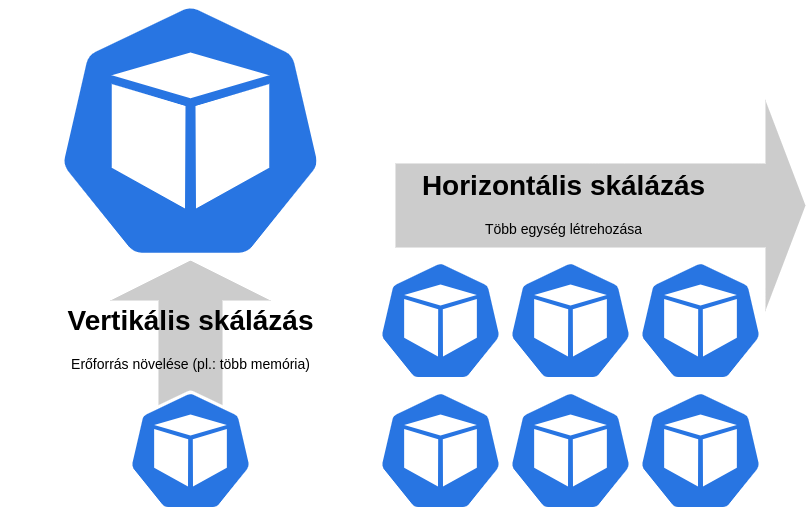
\includegraphics[width=100mm, keepaspectratio]{figures/scaling_types.png}
\caption{Vertikális és horizontális skálázás}
\label{fig:scaling}
\end{figure}

\subsubsection{Automatikus horizontális skálázás}
\label{subsec:hpa}
%----------------------------------------------------------------------------
Egy egyszerű példán keresztül szeretném bemutatni a Kubernetes beépített, automatikus horizontális skálázóját (HPA). Az automatikus skálázónak meg lehet adni, hogy milyen célértéket szeretnénk kapni. Például, hogy a futtatott pod által felhasználható CPU mennyiség milyen szinten legyen kihasználva. Jelenleg ilyen megkötést a memória és processzor felhasználásra lehet tenni, de tetszőlegesen létrehozhatunk saját metrikát is. 

Az algoritmus folyamatosan lekérdezi a metrikák aktuális értékét és \aref{hpa_algo} egyenlet alapján meghatározza az éppen szükséges replika számot. Ezzel a számított értékkel frissíti a pod replika számát, amit így a replikációért felelős kontroller észlel és megpróbálja elérni a kívánt állapotot. Ezzel módszerrel megvalósítható fel- és leskálázás is.

\begin{equation}
\label{hpa_algo}
desiredReplicas = \left\lceil currentReplicas * \frac{currentMetricValue}{desiredMetricValue} \right\rceil
\end{equation}

A folyamat szemléletesebb, ha konkrét példán nézzük meg működését.
Ehhez először létre kellett hozni egy alkalmazást, amit tudunk majd skálázni.
Ehhez egy egyszerű webszervert használtam, ami minden beérkezett kérés esetén egy CPU intenzív műveletet hajt végre. 
Miután létrejött a szükséges \textit{Deployment} és \textit{Service}, utána létre lehetett hozni az automatikus skálázót.
Ennek a forráskódja látható a \ref{hpa_example} kódrészlet tetején.
Be lehet állítani, hogy mi legyen a minimális és maximális replika, ami között lehetősége van skálázni. 
Továbbá definiálni kell egy célértéket is, ami alapján a skálázási döntéseket meg tudja hozni.
A példában látható, hogy $50\%$-os CPU felhasználást szeretnénk elérni.
Fontos, hogy alapvetően a metrikákat a skálázó egy úgynevezett metrika szervertől gyűjti be, amit külön el kell indítani, mert alapértelmezettként nem fut a Kubernetesben. \\

\lstset{caption=Automatikus horizontális skálázás folyamata, label=hpa_example}
\lstinputlisting{figures/hpa_example.sh}

A skálázó létrehozását megtehetjük a kódrészleten látható második parancs kiadásával.
Az erőforrás létrejötte után ki is lehet próbálni.
Ehhez egy \verb+bash+ szkript segítségével állandó forgalmat generálunk és figyeljük, hogyan változik a kapszulák száma és ezzel összefüggően az egyes egységek CPU felhasználása.
Kezdetben $1$ darab pod végezte az összes beérkező kérés kiszolgálását, ami így a célértéknél 3-4-szer több processzort használt.
A korábban mutatott képlet alapján, a felső egész részt vesszük és a jelenlegi replikaszám 4-szeresére skálázunk.


\subsection{Vertikális skálázás}
%----------------------------------------------------------------------------
A skálázási megoldások közül a másik megoldás a \refstruc{fig:scaling} bal oldalán látható. 
Ezt vertikális skálázásnak (másik nevén: scaling up) hívnak. 
Ebben az esetben a kiszolgáló egységek számát nem módosítjuk, hanem az általuk felhasználható erőforrások mennyiségét növeljük.
Ilyen példa, amikor plusz memóriát rakunk a számítógépbe, vagy erősebb processzorra cseréljük a meglévőt. 

Előnye a megoldásnak, hogy a korábbi félévek munkái alatt azt figyeltük meg, hogy a vizsgált alkalmazásaink ezzel a stratégiával azonos erőforrás felhasználás mellett jobb eredményeket értek el.\citep{bscThesis} 

Hátránya, hogy a jelenlegi implementáció szerint minden skálázásnál le kell állítani a futtatott egységet, ami bizonyos szolgáltatás esetén nem túl előnyös, hiszen ezen idő alatt kevesebb egység végzi a beérkező kérések kiszolgálását, illetve azt is jelenti, hogy legalább két pod futása szükséges hozzá.

%Létrehozása esetén figyelni kell, hogy az alá tartozó kapszulák CPU és memória igényeit/limitációit módosítja, ami egy esetlegese HPA alapja lehet.


%TODO : VPA példa kell - nem?

%----------------------------------------------------------------------------
\section{Szolgáltatás minőségi osztályok}
%----------------------------------------------------------------------------

Következőkben szeretném bemutatni a Kubernetes klaszteren belül megjelenő szolgáltatásminőségi osztályokat, illetve azok működését.
Három különböző minőségi osztály létezik jelenleg a Kubernetes implementációjában\citep{KubernetesQoSClasses}. 
Ezen osztályok és hatásaik ismerete hasznos tudást biztosítanak az egyes mérések megtervezéséhez és a kapott eredmények értelmezéséhez.

A Kubernetes minden egyes kapszulához rendel egy minőségi osztályt, amit a beállított erőforrás specifikációkból fog meghatározni.
Tehát, az egyes podok besorolását csak implicit módon lehet definiálni.
Az ütemező számára hasznos információt fog nyújtani, amikor dönteni kell az egyes podok csomóponthoz történő rendeléséről vagy megszüntetéséről.

A kapszulán belüli konkrét osztály meghatározását \aref{get_qos_example} kódrészleten látható módon lehet megtenni.
A \textit{kubectl} alkalmazás \textit{get} és \textit{describe} parancsával is lekérdezhető, de én az előbbit választottam, mert legtöbb esetben bővebb kimenetet kaphatunk, mint a \textit{describe} paranccsal, ugyanis ilyenkor megkapunk minden információt, amit az adott erőforrással kapcsolatban a Kubernetes az \textit{etcd}-ben tárol.

A kimeneten látszik, hogy az érintett erőforrás egy pod, amiben egy darab konténer fut.
A kimenet szükségtelen részét töröltem és csak a számunkra releváns részt hagytam meg.
Látható, hogy egyedül a memória értékre van megkötés, hogy mi legyen a konténer számára maximálisan használható memória mennyiség, ami a példában 170 megabájt. 
Ezzel szemben a pod létrehozásánál létezik megkötés, hogy milyen processzor és memória mennyiségeket szeretne közvetlenül lefoglalni és fixen saját használat alatt tartani.
Könnyen leolvasható, hogy ez a memória esetén 70 megabájt és 100 mCPU processzort jelent.
A számunkra másik fontos részlet már a \textit{status} alatt található.
Itt azok az információk szerepelnek, amiket nem mi definiáltunk és adtunk meg a létrehozás előtt, hanem az erőforrás működése közben változtak.
Többek között ilyenek például, hogy mikor indult el a kapszula, hányszor kellett újraindítani, milyen belső IP címen érhető el illetve a számunka fontos \textit{qosClass} érték is.
Látható, hogy a konkrét példában ez "\textit{Burstable}" értéket kapott. \\

\lstset{caption=Adott kapszula minőségosztályának vizsgálata, label=get_qos_example}
\lstinputlisting{figures/burstable-pod.yaml}

A következő alfejezetekben részletesen bemutatom, az egyes osztályok tulajdonságait, és mi alapján lesznek a kapszulák osztályozva.
Láthatjuk, hogy milyen módon van lehetőségünk az egyes alkalmazások között priorizálni, ezt a Kubernetes hogyan fogja kezelni.
Mindezzel együtt érthetővé válik a korábbi példán látott besorolás is.


\section{Garantált minőségű osztály}
%----------------------------------------------------------------------------

A garantált (\textit{quaranteed}) minőségű szolgáltatás osztály élvezi a legtöbb előnyét a Kubernetes ütemezőnek.
Akkor kerülhet ebbe az osztályba egy adott pod, ha több kritériumnak is megfelel.
A kapszulán belül, minden egyes konténerre érvényesnek kell legyenek, az alábbi megkötések. 
Ezek vonatkoznak a rendes alkalmazás konténerre és az init konténerekre is.

\begin{itemize}
    \item Konténeren belül meg van adva az igényelt és maximálisan használható processzor mennyisége.
    \item Konténeren belül meg van adva az igényelt és maximálisan használható memória mennyisége.
    \item Az igényelt erőforrások és a maximálisan használható erőforrások értékei megegyeznek.
\end{itemize}

A fenti kritériumokhoz kapcsolódóan fontos megjegyezni, azt az érdekes esetet, ami akkor áll elő, ha egy konténerhez mindössze az erőforrások limitációját adjuk meg.
Ebben az esetben automatikusan kerül beállításra az igényelt erőforrás értéke, ami megegyezik a limitációval.
Emiatt hiába nem adunk meg expliciten értéket az igényelt erőforrásokhoz, de kitöltjük a limit értékeket, akkor is garantált szolgáltatás osztályba fog kerülni az adott pod.

Ezen kapszulák olyan csomópontokra kerülnek ütemezésre, amik rendelkeznek elegendő erőforrással, illetve a bennük futtatott konténerek lesznek a kevés erőforrás miatt utoljára leállítva.

\section{Börsztölhető minőségű osztály}
%----------------------------------------------------------------------------
% ToDo: börsztölhető lehet nem a legjobb kifejezés
A börsztölhető (\textit{burstable}) kapszulák besorolását elég széleskörűen lehet meghatározni.
Leginkább azt lehet mondani, hogy ide tartoznak azok a podok, amik valami miatt nem teljesítik a garantált szolgáltatás osztályba tartozó kritériumokat, azonban valamilyen erőforrás foglalás meg van adva.
Tipikusan ilyen szituáció, amikor különböző értékek vannak megadva az igényelt és a maximálisan használható erőforrások mennyisége között.
Akkor is ide kerül besorolásra egy kapszula, ha több konténer közül valamelyik nem teljesíti a garantált osztály elvárásait.

Ezen podokat igyekszik az ütemező a rendelkezésre álló információi alapján a számukra legjobb csomópontra osztani, de nem garantálható ennek a sikere.
Ez abból fakad, hogy legtöbb esetben kevesebb információval rendelkezik róluk, mint a garantált osztályban, ahol minden érték adott volt.

Amikor elfogynak a csomópont által használható erőforrások és nincsen több legjobb szándék minőségű osztályba tartozó pod, akkor ezen podok kerülnek leállításra. 
Ezzel is védve a garantált osztályú kapszulákat.

\section{Legjobb szándék minőségű osztály}
%----------------------------------------------------------------------------
Legalacsonyabb prioritási szinttel a legjobb szándék (\textit{best effort}) minőségi osztály rendelkezik a felsoroltak közül, amire már a neve is utal.
Ide kerülnek az olyan kapszulák, ahol semelyik konténernek nincsen beállítva erőforrásra vonatkozó információ.
Tehát nincs megkötés a maximális használatra és nincs megkötés a minimálisan szükséges erőforrásra sem.

Ebben az esetben rendelkezik az ütemező a legkevesebb információval a kapszuláról, ami miatt nem is garantálható, hogy olyan csomóponton kerül elindításra, ahol elegendő erőforrás áll az alkalmazás rendelkezésére.

Ebbe a kategóriába tartozó podok annyi erőforrást használhatnak, amennyi rendelkezésre áll az adott csomóponton.
Emiatt felmerül a veszélye, hogy a többi alkalmazás elől fogja elhasználni a szükséges erőforrásokat. 
Ezzel magyarázható, hogy az osztályba tartozó podok lesznek először leállítva, amikor fogytán van a csomóponton elérhető erőforrások mennyisége.
\\
\\
A fentebb írtak miatt körültekintően kell eljárni az erőforrások szabályozása közben, hiszen ezáltal lehetőségünk van priorizálni az alkalmazásainkat.
